\documentclass[nynorsk]{mnt}

\usepackage{graphicx}   % to import PNG, JPEG and PDF graphics

\conference{MNT-konferansen 2019, 28.-29. mars, Tromsø}

\title{\LaTeX\ til MNT-konferansen}
\author{Hans Georg Schaathun,
\emph{NTNU --- Noregs Teknisk-Naturvitskaplege Universitet}}

\begin{document}
\maketitle

\begin{abstract}
   Når me ser på tradisjonelle eksamensoppgåver i emnet ser me at 
   studentane har rett. Ferdigheitsmåla står i fokus, og kunnskaps-
   og kompetansemåla har vore gløymde både i undervisinga og på
   eksamen tidlegare år, mao.\ eit klart brot med 
   \emph{constructive alignment} \citep{biggs11a} 
   eller samstemt undervisning.
   Dette problemet kan me òg kjenna igjen i mange andre matematikkemne.
\end{abstract}

\section{Innleiing}

Høge stryktal i matematikk er ei velkjend utfordring frå mange studium.
Emne- og studieansvarlege landet over freistar 
stadig nye tiltak for å auka gjennomstrauminga.
Matematikken er prega av sterke tradisjonar og forventingar om kva
studentane bør kunne.

\begin{table}
\centering
  \caption{Karakterfordeling.}
  \begin{tabular}{l|r|r|r|r|r|r|}
     & \multicolumn{1}{c|}{A}
     & \multicolumn{1}{c|}{B}
     & \multicolumn{1}{c|}{C}
     & \multicolumn{1}{c|}{D}
     & \multicolumn{1}{c|}{E}
     & \multicolumn{1}{c|}{F} \\
  \hline
  2018 & 1 & 7 & 28 & 24 & 29 & 49 \\
  \hline
  2018 &
  \num{0.72}\% &
  \num{5.1}\% &
  \num{20.3}\% &
  \num{17.4}\% &
  \num{21.0}\% &
  \num{35.5}\%  \\
  \hline
  2017 &
  \num{1.5}\% &
  \num{5.1}\% &
  \num{15.4}\% &
  \num{14.7}\% &
  \num{20.6}\% &
  \num{42.6}\% \\
  \hline
  \end{tabular}
  \label{tab:grade}
\end{table}


Tabell~\ref{tab:grade} viser eit døme på tabell.

\begin{figure}
\begin{center}
  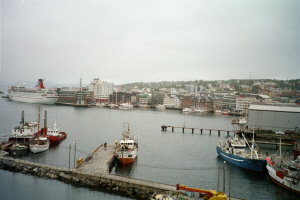
\includegraphics[width=0.6\textwidth]{tromso}
\end{center}
  \caption{Overblikk over Tromsø; teke frå broen mot Tromsdalen.
    Gustav Foseid (User:Gustavf on en.wikipedia)
    Juli 2003.
    Lisensiert under \emph{GNU Free Documentation License}.
    }
  \label{fig}
\end{figure}

Eit par andre døme:
\begin{itemize}
  \item 
Korte evalueringsspørsmål i førelesingane gjennom eit
      quizverkty \citep{hgs2018udit}.
   \begin{itemize}
     \item nøsting er lov
     \item ... men er det riktig kulesymbol?  Det må redaktøren svara på.
   \end{itemize}
  \item 
Figur~\ref{fig} viser Tromsø, der neste MNT-konferanse vert arrangert.
\end{itemize}

... og nummererte lister ...
\begin{enumerate}
  \item 
    \cite{biggs11a} sa at ...
  \item Punkt 2.
\end{enumerate}

Somme tider treng me sitat, t.d.\
\begin{quote}
Høge stryktal i matematikk er ei velkjend utfordring frå mange studium.
Emne- og studieansvarlege landet over freistar 
stadig nye tiltak for å auka gjennomstrauminga.
Matematikken er prega av sterke tradisjonar og forventingar om kva
studentane bør kunne.

\raggedleft\emph{Anonym matematikklærar}
\end{quote}
eller 
\begin{quotation}
Høge stryktal i matematikk er ei velkjend utfordring frå mange studium.
Emne- og studieansvarlege landet over freistar 
stadig nye tiltak for å auka gjennomstrauminga.
Matematikken er prega av sterke tradisjonar og forventingar om kva
studentane bør kunne.

Sitatet kan gjerne ha fleire avsnitt.

\raggedleft\emph{Anonym matematikklærar}
\end{quotation}
Bruk \verb.quotation. når sitatet har meir enn eitt avsnitt, og 
\verb.quote. når det anten er eitt avsnitt eller ein serie med 
einskildliner.

%\footnotesize
\bibliographystyle{apalike}
\bibliography{template}

\end{document}
